\documentclass[a4paper,12pt]{report}
\usepackage
[
a4paper,
left=4cm,
right=2.5cm,
top=3cm,
bottom=4cm,
]
{geometry}
\usepackage[czech]{babel}
\usepackage[utf8]{inputenc}
\usepackage[T1]{fontenc}
%\usepackage{hyperref}
\usepackage{xcolor} % barevný text - vyšedění
\usepackage{amsmath}
\usepackage{amssymb}
\usepackage{amsthm}
%\usepackage[toc,page]{appendix}
\usepackage{mdframed}
\usepackage{graphicx}
%\usepackage{subfigure}  % abych mohl dát 2 obrázky vedle sebe
\usepackage[font=footnotesize,labelfont=bf,justification=centering]{caption} % 2 obrázky vedle sebe, nastavuje font a centruje caption nad tabulkama a u obrázků
\usepackage[font=scriptsize]{subcaption}
\captionsetup{font=footnotesize}

%\usepackage{titlesec}
\usepackage{icomma} %nedělá za čárkou v číslech automaticky mezeru
\usepackage{url}
\usepackage{float}
\usepackage{enumerate} % hezky číslované listy (např. římská čísla)
%\usepackage[justification=centering]{caption} 

\usepackage{listings}
\usepackage{booktabs}

\newtheorem{theorem}{Věta}[chapter]
\newtheorem*{theoremnon}{Věta}
\newtheorem{lemma}{Lemma}[chapter]
\newtheorem{corollary}{Důsledek}[chapter]
%\theoremstyle{definition}
\newtheorem{definition}{Definice}[chapter]
\newtheorem*{defnon}{Definice}
\newtheorem{problem}{Úloha}[chapter]
\theoremstyle{remark}
\newtheorem{remark}{Poznámka}[chapter]

\renewcommand\qedsymbol{$\blacksquare$} % plný čtvereček za důkazem



\setlength{\topmargin}{-.25in}
\setlength{\parindent}{0pt}
\setlength{\parskip}{0.5\baselineskip}

%\usepackage{titlesec}
%\titleformat{\chapter}
%{\normalfont\LARGE}{\thechapter}{1em}{}
%\titlespacing*{\chapter}{0pt}{3.5ex plus 1ex minus .2ex}{2.3ex plus .2ex}

% Obecná definice pro styl nadpisů kapitol, sekcí atd. 
\usepackage{titlesec, blindtext, color}
\definecolor{gray75}{gray}{0.75}
\newcommand{\hsp}{\hspace{20pt}}

% Definice stylu pro chapter title
\titleformat{\chapter}[hang]{\Huge\bfseries}{\thechapter\hsp\textcolor{gray75}{|}\hsp}{0pt}{\Huge\bfseries}
% Definice stylu pro chapter title - bez číslování
\titleformat{name=\chapter,numberless}[hang]{\Huge\bfseries}{\hsp\textcolor{gray75}{|}\hsp}{0pt}{\Huge\bfseries}
% Definice stylu pro section title
\titleformat{\section}[hang]{\Large\bfseries}{\thesection\hsp\textcolor{gray75}{|}\hsp}{0pt}{\Large\bfseries}

\definecolor{identifiercolor}{rgb}{.4,.6,.56}
\definecolor{stringcolor}{gray}{0.5}
\definecolor{inactivecolor}{rgb}{0.15,0.15,0.5}
\usepackage{listings}
\lstset{basicstyle={\footnotesize\def\fvm@Scale{.85}\fontfamily{fvm}\selectfont},
	breaklines=true,
	escapeinside={\%*}{*)},
	keywordstyle={\bfseries\color{inactivecolor}},
	stringstyle={\bfseries\color{stringcolor}},
	identifierstyle={\bfseries\color{identifiercolor}},
	language=Mathematica,
	otherkeywords={DiscretizeRegion},
	showstringspaces=false}
\renewcommand{\lstlistingname}{Listing}


%%%%%%%% per partes
\ExplSyntaxOn
\NewDocumentCommand{\byparts}{O{0pt}m}
{
	\keys_set:nn { elisabeth/byparts } { #2 }
	\elisabeth_byparts:n { #1 }
}

\keys_define:nn { elisabeth/byparts }
{
	x  .tl_set:N = \l__elisabeth_byparts_u_tl,
	x' .tl_set:N = \l__elisabeth_byparts_up_tl,
	y  .tl_set:N = \l__elisabeth_byparts_v_tl,
	y' .tl_set:N = \l__elisabeth_byparts_vp_tl,
}

\cs_new_protected:Nn \elisabeth_byparts:n
{
	\begin{vmatrix}\,\begin{aligned}
			x\hphantom{'} &= \l__elisabeth_byparts_u_tl
			&
			y' &= \l__elisabeth_byparts_vp_tl
			\\[#1]
			x' &= \l__elisabeth_byparts_up_tl
			&
			y\hphantom{'} &= \l__elisabeth_byparts_v_tl
		\end{aligned}\,\end{vmatrix}
}

\ExplSyntaxOff
%%%%%%%%%%%%%%%%%


\title{
	{
\includegraphics[width=\linewidth]{FAV_logo.jpg}}\\[2cm]
	{Lineární řešiče v OpenFOAM}\\	
	{\small{Semestrální práce}}\\
	{\small{KMA/PVM}}\\
}

\author{Jan Půlpán}


\begin{document}
	\maketitle

	{\let\clearpage\relax \chapter{Teoretický úvod}}

	OpenFOAM je sada výpočetních nástrojů pro numerické simulace CFD (computational fluid dynamics) problémů, tedy problémů zabývajících se prouděním tekutin, vedením tepla a podobných procesů. OpenFOAM využívá k hledání řešení metody konečných objemů (FVM). 
	
	FVM je numerická metoda na řešení parciálních diferenciálních rovnic na dané geometrii transformované na síť nepřekrývajích se elementů (konečných objemů). Diskretizací úlohy získáme soustavu lineárních algebraických rovnic v neznámé $\boldsymbol{x}$ pro každou ze sledovaných proměnných. Soustava je tvaru
	\begin{equation}
		\boldsymbol{A}\boldsymbol{x} = \boldsymbol{b},
		\label{eq:linear_set}
	\end{equation}
	kde $\boldsymbol{A}$ je regulární matice popisující diskretizovaný model, $\boldsymbol{x}$ vektor závislé proměnné a $\boldsymbol{b}$ vektor pravé strany obsahující všechny zdroje, okrajové podmínky a všechny komponenty, které nelze linearizovat. 
	
	Zabývat se budeme jen posledním článkem řetězce, tedy lineárními řešiči algebraických rovnic. Na testovací úloze si ukážeme vhodnost jednotlivých řešičů a budeme sledovat vliv parametrů na konvergenci řešení. Dále budeme o lineárních řešičích mluvit jen jako o  \uv{řešičích}, pokud nebude hrozit záměna kontextu.
	
	Obecně lze soustavu lineárních rovnic řešit buď přímými nebo iteračními řešiči. Úlohy CFD jsou většinou silně nelineární a proto není jejich řešení pomocí přímých řešičů snadné a vyžaduje větší výpočetní výkon.
	
	Přímé řešiče hledají přesné řešení pomocí inverzní matice $\boldsymbol{A} ^{-1}$ ve formě
$$ \boldsymbol{x} = \boldsymbol{A}^{-1} \boldsymbol{b}.$$  
Většina přímých metod je založna na Gaussově eliminici a případné transformaci úlohy na úlohu se stejným řešením ale snadněji řešitelnou, například pomocí LU nebo DILU rozkladu.

	I když přímé řešiče naleznou vždy přesné řešení v konečném počtu kroků, výpočetní náročnost je extrémní. Inverzi $\boldsymbol{A} ^{-1}$ není výpočetně levné nalézt a proto se většinou používají přibližné řešiče iterační. Výhodou těchto metod je mnohem menší výpočetní náročnost i náročnost na paměť. Pomocí iterací počítáme posloupnost řešení $\boldsymbol{x}^{(n)}$, která za daných podmínek konverguje k řešení $\boldsymbol{x}$.  Nejčastěji využívané iterační řešiče jsou Gaussova-Seidelova metoda, metody Krylovových prostorů (kam patří například metoda sdružených gradientů) a víceúrovňové metody.
	
	Iterační metody obecně měří chybu aproximace řešení v každém kroku pomocí reziduí, tedy dosazením aproximovaného řešení do původních rovnic a vypočtením rozdílu oproti pravé straně $\boldsymbol{b}$. Reziduum $\boldsymbol{r} ^{(n)} $ definujeme jako 

	\begin{equation}
		\boldsymbol{r} ^{(n)} = \boldsymbol{b}-\boldsymbol{A} \boldsymbol{x}^{(n)}.
		\label{eq:residuum}
	\end{equation} 

Zastavení řešiče je pak definováno obecně jako pokles residua pod nastavenou hodnotu

$$\Vert{\boldsymbol{r}^{(n)}}\Vert < \epsilon.$$
	
	OpenFOAM obsahuje kromě přímých řešičů hlavně iterační řešiče pomocí gradientních metod, víceúrovňových metod a řešiče pomocí smootherů (vyhlazovačů).
	
\textbf{Gradientní metody} jsou založeny na tom, že úlohu \eqref{eq:linear_set} lze přeformulovat na úlohu minimalizace kvadratické funkce
\begin{equation}
	\boldsymbol{Q}(\boldsymbol{x}) = \frac{1}{2} \boldsymbol{x}^T \boldsymbol{A} \boldsymbol{x}-\boldsymbol{b}^T \boldsymbol{x} + \boldsymbol{c}.
	\label{eq:quad_func}
\end{equation}
V případě symetrické a positivně definitní matice $\boldsymbol{A}$ je iterační metoda řešení úlohy \eqref{eq:linear_set} definována vztahem
\begin{equation}
	\boldsymbol{x}^{(n+1)} = \boldsymbol{x}^{(n)} + \alpha^{(n)} \left( \boldsymbol{\delta} \boldsymbol{x}^{(n)} \right),
	\label{eq:grad_iter}
\end{equation}
kde $\alpha^{(n)}$ je relaxační faktor (viz níže) a $\boldsymbol{\delta} \boldsymbol{x}^{(n)}$ je člen minimalizující funkci \eqref{eq:quad_func}, který lze získat například metodou největšího spádu, kdy použijeme jako minimalizující prvek gradient $\nabla Q(\boldsymbol{x}^{(n)})$. To ale často vede k oscilacím okolo minima a proto se většinou používá metoda sdružených gradientů. Ta pracuje s posloupností $N$ směrů  $\boldsymbol{d}^{(0)}, \boldsymbol{d}^{(1)}, \boldsymbol{d}^{(2)} \cdots \boldsymbol{d}^{(N-1)}$ takových, že splňují
\begin{equation*}
	\left(\boldsymbol{d}^{(n)}\right)^T\boldsymbol{A} \boldsymbol{d}^{(m)} = 0
\end{equation*}
a jsou tedy $\boldsymbol{A}$-ortogonální. Iterační metoda je popsaná následujícím vztahem

\begin{equation*}
	\boldsymbol{x}^{(n+1)} = \boldsymbol{x}^{(n)} + \alpha^{(n)} \boldsymbol{d}^{(n)}.
	\label{eq:grad_cg}
\end{equation*}

V případě, že není matice $\boldsymbol{A}$ symetrická, lze použít metodu bi-sdružených gradientů, která konverguje úlohu na úlohu se symetrickou maticí následovně.

\begin{equation}
	\begin{bmatrix}
		0 & \boldsymbol{A}\\
		\boldsymbol{A}^T & 0
	\end{bmatrix}
	\begin{bmatrix}
		\hat{\boldsymbol{x}}\\
		\boldsymbol{x}
	\end{bmatrix} =
	\begin{bmatrix}
		\boldsymbol{b}\\
		0
	\end{bmatrix}
\end{equation}

%%% https://astra.nti.tul.cz/~petr.sidlof/vyuka/NMPT/pr05%20-%20Reseni%20linearnich%20systemu%20a%20paralelizace.pdf

V součastnosti asi nejpoužívanější jsou \textbf{víceúrovňové} (multigrid) metody. Ty odstraňují základní problém Krylovovských metod, tedy vysokou náročnost na hardware už pro středně velké úlohy. Základní myšlenkou je využití několika různě velkých sití. Ty jemnější pro detailnější řešení a odstranění vysokofrekvenčních chyb, hrubší pak pro rychlé odstranění nízkofrekvenčních chyb, které nejsou na jemnějších sítích rozpoznatelné a proto často prodlužují konvergenci. 

Víceúrovňová metoda postupuje v následujících krocích:
\begin{enumerate}
	\item několik kroků iterační metody (např. Gauss-Seidel) na jemné síti - pre-smoothing,
	\item projekce na hrubší síť - restriction,
	\item řešení na hrubé síti (na velmi hrubé síti je možné použít i přímý řešič), odstranění nízkofrekvenčních chyb,
	\item projekce zpět na jemnou síť - prolongation,
	\item několik kroků iterační metody na vyhlazení vysokofrekvenčních chyb - post-smoothing.
\end{enumerate}

Úrovní sítí je většinou více než 2 a podle způsobu přechodů (restriction a prolongation fáze) mezi nimy se mluví o tzv. V-cyklech, W-cyklech, případně F-cyklech. Víceúrovňové metody se využívají ve 2 variantách:
\begin{itemize}
	\item geometrické - na úrovni sítě, využívá informaci o sousedních elementech,
	\item algebraické - na úrovni matice, bez znalosti gometrie, je univerzální pro jakékoliv problémy.
\end{itemize}
	
%	\begin{equation}
%		\boldsymbol{x^{(k+1)}} = \boldsymbol{M}^{-1}(\boldsymbol{N}\boldsymbol{x^{(k)}} + \boldsymbol{b})
%		\label{eq:stat_iter}
%	\end{equation}

%	Pevný bod operátoru \eqref{eq:stat_iter} je pak přesným řešením soustavy \eqref{eq:linear_set}.  
	
%	Druhou používanou metodou iteračních řešičů jsou metody Krylovových podprostorů. Hledáme tak přibližné řešení v podprostorech s rostoucí dimenzí generovaných čtvercovou maticí $\boldsymbol{A}$ a vektorem $\boldsymbol{b}$. Krylovův podprostor $r$tého řádu je definován jako 
%	$$\mathcal{K}_r(\boldsymbol{A},\boldsymbol{b}) = \textrm{span}\{\boldsymbol{b}, \boldsymbol{Ab}, \boldsymbol{A}^2\boldsymbol{b}, \dots, \boldsymbol{A}^{r-1}\boldsymbol{b}\}.$$
%	TROCHU LÍP POPSAT, KOUKNOUT DO NA
		
	Iterační metody řešení lineárních algebrických rovnic často využívají \textbf{předpodmínění} (preconditiong). To převede úlohu do tvaru s ekvivalentním řešením ale lepšímy spektrálnímy vlastnostmi matice soustavy.  Při levém předpodmínění (existuje i pravé a centrální) předpokládáme soustavu ve tvaru
	$$\boldsymbol{P}^{-1}\boldsymbol{A}\boldsymbol{x} =\boldsymbol{P}^{-1}\boldsymbol{b},$$
	kde $\boldsymbol{P}$ je předpodmiňovač. Ten zajistí, že konvergence předpodmíněného systému je rychlejší než bez něj. Při hledání předpodmiňovače $\boldsymbol{P}$ je často uvažována nějaká snadno invertovatelná aproximace matice $\boldsymbol{A}$. Nejjednodušší volbou je tak $\boldsymbol{P} = \boldsymbol{I}$, což ovšem vede k nepodmíněnému problému. Ideální je naopak $\boldsymbol{P} = \boldsymbol{A}$, to ovšem znamená, že inverze předpodmiňovače je stejně náročná jako původní matice. Často se tak volí různé rozklady matice $\boldsymbol{A}$, jako jsou LU, ILU nebo DILU rozklady.
	
	Pro zrychlení konvergence se u iteračních řešičů využívá tzv. \textbf{vyhlazovač} (smoother), pro který lze používat např. základní Jacobiho, nebo Gaussovu-Seidelovu metodu. Po každé iteraci řešiče metody se pustí několik kroků vybraného vyhlazovače, který \uv{vyhladí} špičky v reziduu a tím i sníží jeho normovanou hodnotu. Na rozdíl od předpodmínění dokáže vyhlazovač snížit počet kroků nezávisle na velikosti sítě. Pro příklad uveďme iterační vztah pro Gaussův-Seidelův vyhlazovač, kde $\boldsymbol{L}$ je dolní trojúhelníková část matice $\boldsymbol{A}$.
	
	\begin{equation}
		\boldsymbol{x^{(k+1)}} = \boldsymbol{x^{(k)}}+\boldsymbol{L}^{-1}(\boldsymbol{b} -  \boldsymbol{A}\boldsymbol{x^{(k)}}),
		\label{eq:gs_smoother}
	\end{equation}

Další vyhlazovače jsou pak založeny na principu LU, DILU, nebo Choleského rozkladu.
	
	Aby se zlepšila stabilita numerického řešiče, doporučuje se využít \textbf{relaxaci} metody. Pomocí relaxačního faktoru $\alpha, 0 < \alpha \leq 1 $, limituje relaxace změnu řešení mezi jednotlivými iteracemi dle vztahu \eqref{eq:grad_iter}. Pokud je   $\alpha = 1$ , žádná relaxace se neuplatňuje, $\alpha = 0$ znamená žádnou změnu mezi jednotlivými kroky.   Optimální $\alpha$ je dostatečně malé, aby zabránilo oscilacím v numerických výpočtech a zároveň dostatečně velké, aby nezpomalovalo nadměrně konvergenci. 
	
	{\let\clearpage\relax \chapter{Lineární řešiče v OpenFOAM}}

OpenFOAM obsahuje kromě základního přímého řešiče \texttt{diagonalSolver} tři základní typy řešičů:
\begin{enumerate}
	\item řešiče typu sdružených gradientů 
	\item víceúrovňové řešiče
	\item řešiče založené na vyhlazovači

\end{enumerate}

Konkrétní řešiče jsou popsány v tabulce \ref{table:solvers}.

\begin{table}[H]
	\centering
	\caption{řešiče v rámci OpenFOAM}
	\renewcommand{\arraystretch}{1.7}
	\begin{tabular}{*3l}
		\toprule
		\textbf{Řešič} & \textbf{Označení}&\textbf{Matice $\boldsymbol{A}$}\\
		\midrule
		{\small Předpodmíněné sdružené gradienty}& PCG& sym\\
		{\small Předpodmíněné bi-conjugate gradient}& PBiCG&asym \\		
		{\small Stabilizované předpodmíněné (bi-)conjugate gradient}& PBiCGStab&sym/asym  \\
		{\small Řešič používající vyhlazovač}& smoothSolver&sym/asym \\
		{\small Víceúrovňový řešič}& GAMG&sym/asym  \\
		{\small Diagonální přímý řešič}& 	diagonal \\
	
		\bottomrule
	\end{tabular}
	
	\label{table:solvers}
\end{table}
		
To který řešič je možné použít je závislé na matici $\boldsymbol{A}$ a tom, jestli je symetrická nebo nesymetrická. Symetrie $\boldsymbol{A}$ samozřejmě závisí na rovnicích, které chceme řešit. V případě, že zvolíme nesprávný řešič vzhledem k symetričnosti matice $\boldsymbol{A}$ OpenFOAM sám volbu opraví.

Doporučeným řešičem v OpenFOAM je, jak jsme již uvedli v teoretické části obecně,  víceúrovňový řešič GAMG (geometric-algebraic multi-grid). Řešičem o kterém jsme dosud nemluvili je řešič založený na vyhlazovači, kdy vybraný smoother slouží nejen k vyhlazení, ale i k řešení soustavy.  Většinou je nejlepší volbou Gauss-Seidel.

Během jednotlivých iterací je v OpenFOAM reziduum vyhodnocováno pomocí vztahu \eqref{eq:residuum}. Každý řešič má k reziduu trochu jíný přístup, obecně ale dochází k normalizaci a škálování rezidua $\boldsymbol{r}$ vztahy

$$n = \sum \left( | \boldsymbol{A} \boldsymbol{x} - \boldsymbol{A} \overline{\boldsymbol{x}} | + | \boldsymbol{b} - \boldsymbol{A} \overline{\boldsymbol{x}} | \right),$$
$$\boldsymbol{r} = \frac{1}{n} \sum | \boldsymbol{b} - \boldsymbol{A} \boldsymbol{x} |,$$

kde $\overline{\boldsymbol{x}}$ je průměrný vektor řešení.  

Pro každý typ řešice je třeba nastavit zastavovací parametr pro velikost rezidua (\texttt{tolerance}) a také relativní toleranci (\texttt{relTol}) což je poměr aktuálního rezidua a počátečního rezidua před začátkem iterace. Lineární řešič se následně zastaví pokud je splněna alespoň jedna z těchto podmínek:
\begin{enumerate}
	\item reziduum je menší než nastavená \texttt{tolerance},
	\item relativní tolerance je menší než nastavená \texttt{relTol},
	\item je dosaženo nastaveného maximálního počtu iterací \texttt{maxIter}.
\end{enumerate}


%Metoda sdružených gradientů (conjugent gradients) - PCG. PBiCG, PBiCGStab

%Metoda sdružených gradientů (CG) je iterační algoritmus řešení soustav lineárních rovnic, který využívá sdružených směrů a vyžaduje symetrickou matici (postivně definitní) matici $\boldsymbol{A}$. Proto vznikla i metoda "bi-conjugate gradients" (dvojitých sdružených směrů), která pracuje s asymetrickými maticemi. OpenFoam obsahuje řešiče PCG a PBiCG s implementací těchto řešičů. Obě varianty jsou předpodmíňěné. Navíc je obsažen i PBiCGStab řešič, který umí pracovat se symetricvkou i nesymetrickou maticí $\boldsymbol{A}$.

U většiny řešičů je pak volitlně nastaven předpodmičovač případně vyhlazovač. Podporované předpodmiňovače jsou v tabulce \ref{table:preconditioners} a vyhlazovače v tabulce \ref{table:smoothers}.

\begin{table}[H]
	\centering
	\caption{Předpodmiňovače implementované v OpenFOAM}
	\renewcommand{\arraystretch}{1.7}
	\begin{tabular}{*2l}
		\toprule
		\textbf{Předpodmiňovač} & \textbf{Označení}\\
		\midrule
		{\small Diagonal incomplete-Cholesky (symetrický)}& DIC\\
		{\small Faster diagonal incomplete-Cholesky (DIC with caching)	}& FDIC \\		
		{\small Diagonální neúplný LU rozklad}& DILU  \\
		{\small Diagonální přímý}& diagonal \\
		{\small Víceúrovňový předpodmiňovač}& GAMG  \\
		\bottomrule
	\end{tabular}
	
	\label{table:preconditioners}
\end{table}

\begin{table}[H]
	\centering
	\caption{Vyhlazovače implementované v OpenFOAM}
	\renewcommand{\arraystretch}{1.7}
	\begin{tabular}{*2l}
		\toprule
		\textbf{Vyhlazovačč} & \textbf{Označení}\\
		\midrule
		{\small DIC Gauss Seidel vyhlazovač}& DICGaussSeidel\\
		{\small DIC vyhlazovač}& DIC\\		
		{\small DILU vyhlazovač}& DILU \\		
		{\small Gaussův-Seidelův vyhlazovač}& GaussSidel  \\
		{\small Symetrický Gaussův-Seidelův vyhlazovač}& symGaussSeidel \\
		\bottomrule
	\end{tabular}
	
	\label{table:smoothers}
\end{table}

	{\let\clearpage\relax \chapter{Porovnání řešičů}}
	
	Lineární řešiče porovnáme na konkrétní úloze stacionárního proudění v lopatkové mříži. Zachováme přitom jednotné parametry nastavení úlohy až na nastavení jednotlivých lineárních řešičů. Zajímat nás bude konvergence řešení a výpočetní náročnost. Zadání úlohy je na obrázku \ref{fig:zadani}, který definuje geometrii úlohy i okrajové podmínky. 
	
	\begin{figure}[H]
		\centering
		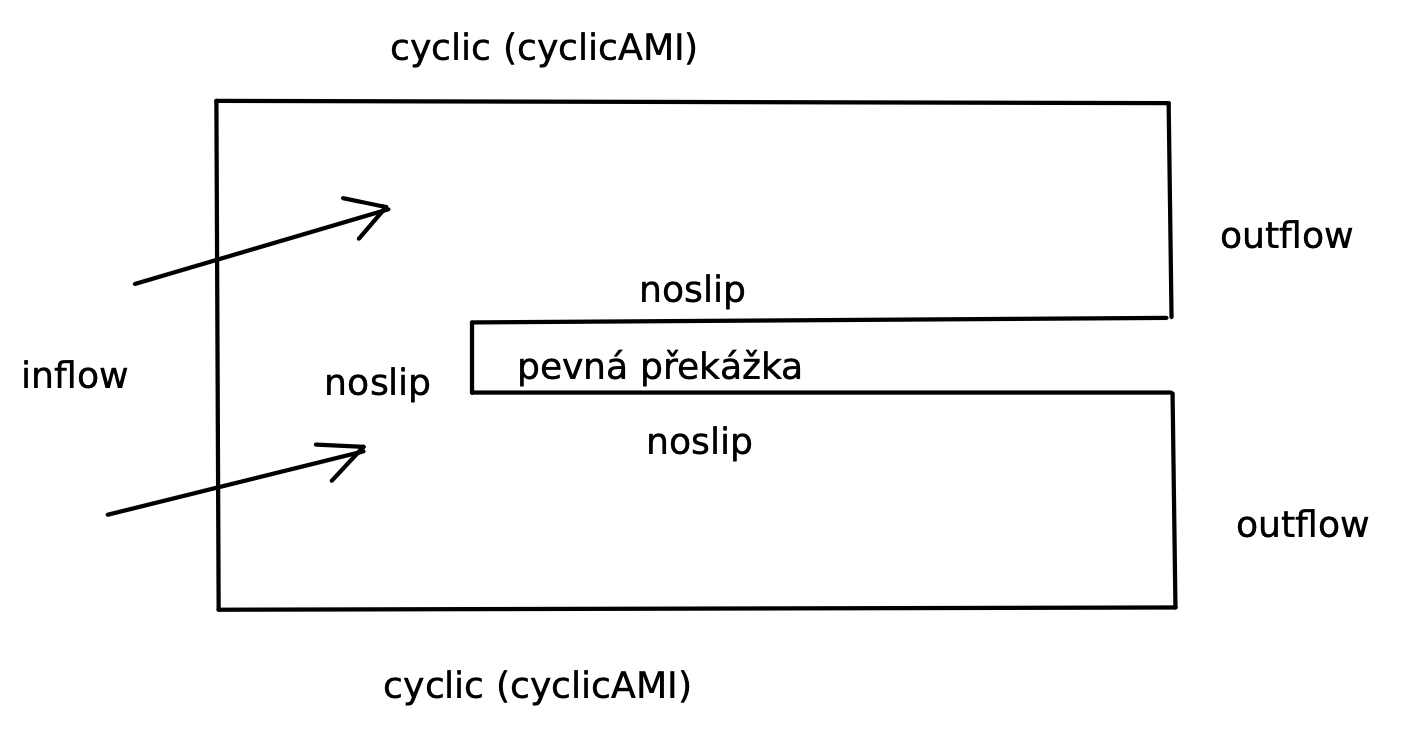
\includegraphics[width=1\linewidth]{zadani.png}
		\caption{Popis řešeného modelu}
		\label{fig:zadani}
	\end{figure}


Nejprve musíme definovat síť na které budeme naši úlohu řešit. Úloha je v 2D, ale OpenFOAM řeší vše ve 3D. Třetí souřadnici tedy nastavíme minimální, jen jako jednu buňku, a budeme ji ve výsledcích vlastně ignorovat.  Nejvíce se toho bude dít kolem \uv{vykousknuté} části a proto v těchto místech síť uděláme hustší jak je vidět na obrázku \ref{fig:pvmesh-detail}. Celá síť je pak na obrázku \ref{fig:pvmesh} a obsahuje celkem $108800$ jednotlivých buněk, na kterých budeme úlohu numericky integrovat. Konkrétní definice je v souboru \texttt{blockMeshDict} v příloze \ref{app:blockmeshdict}.

\begin{figure}[H]
	\centering
	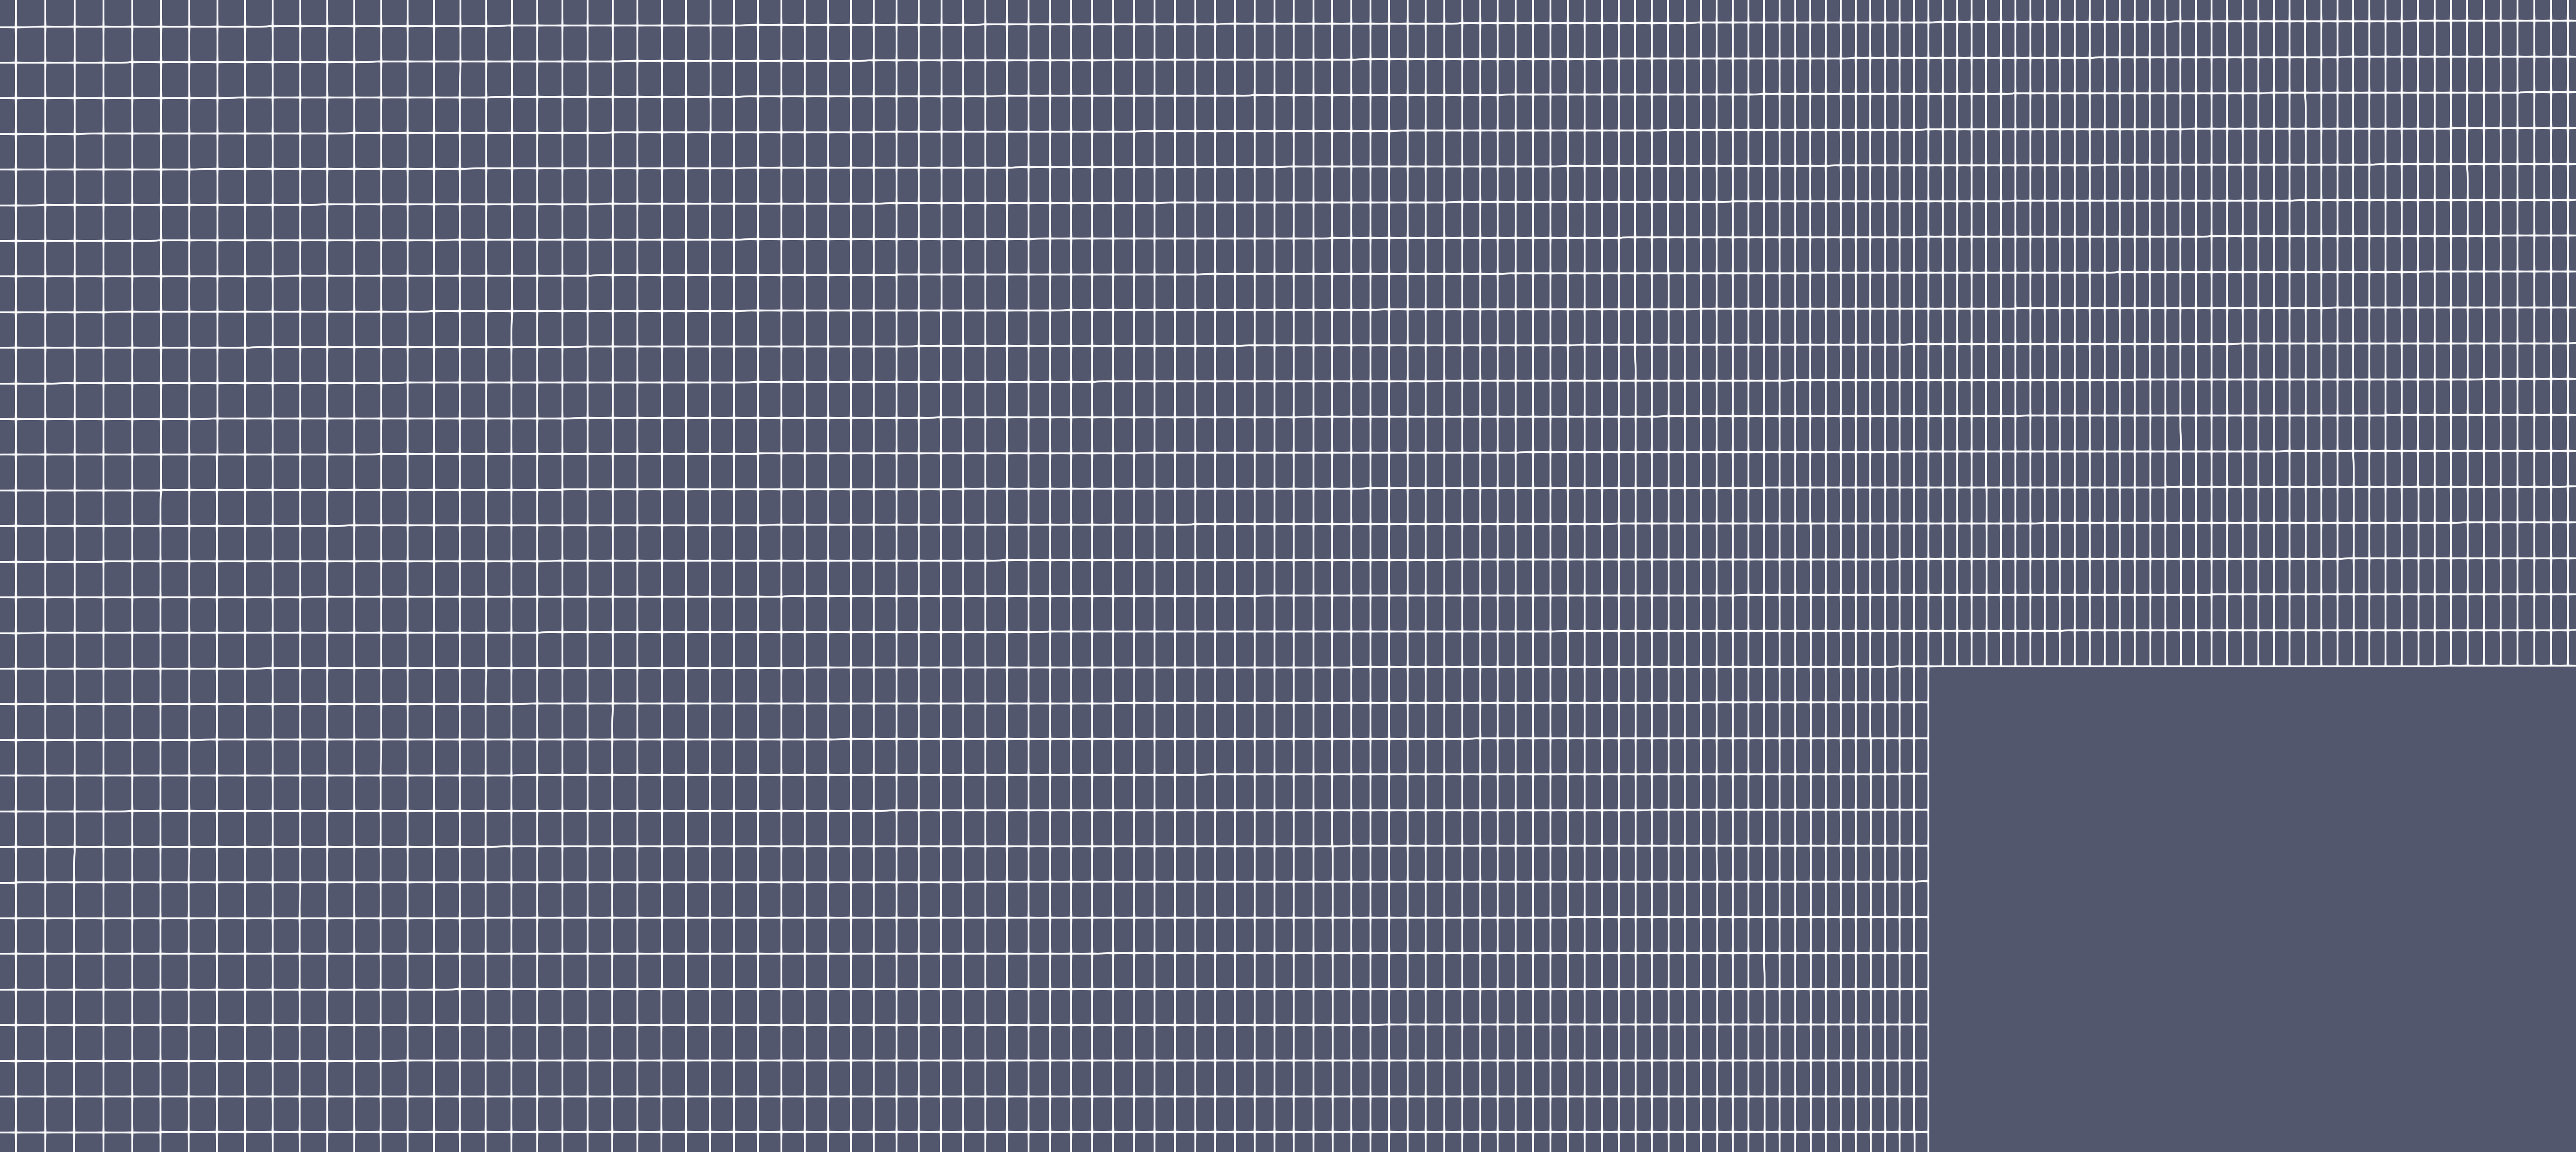
\includegraphics[width=1\linewidth]{pv-mesh-detail.png}
	\caption{Detail sítě řešeného modelu}
	\label{fig:pvmesh-detail}
\end{figure}



\begin{figure}[H]
	\centering
	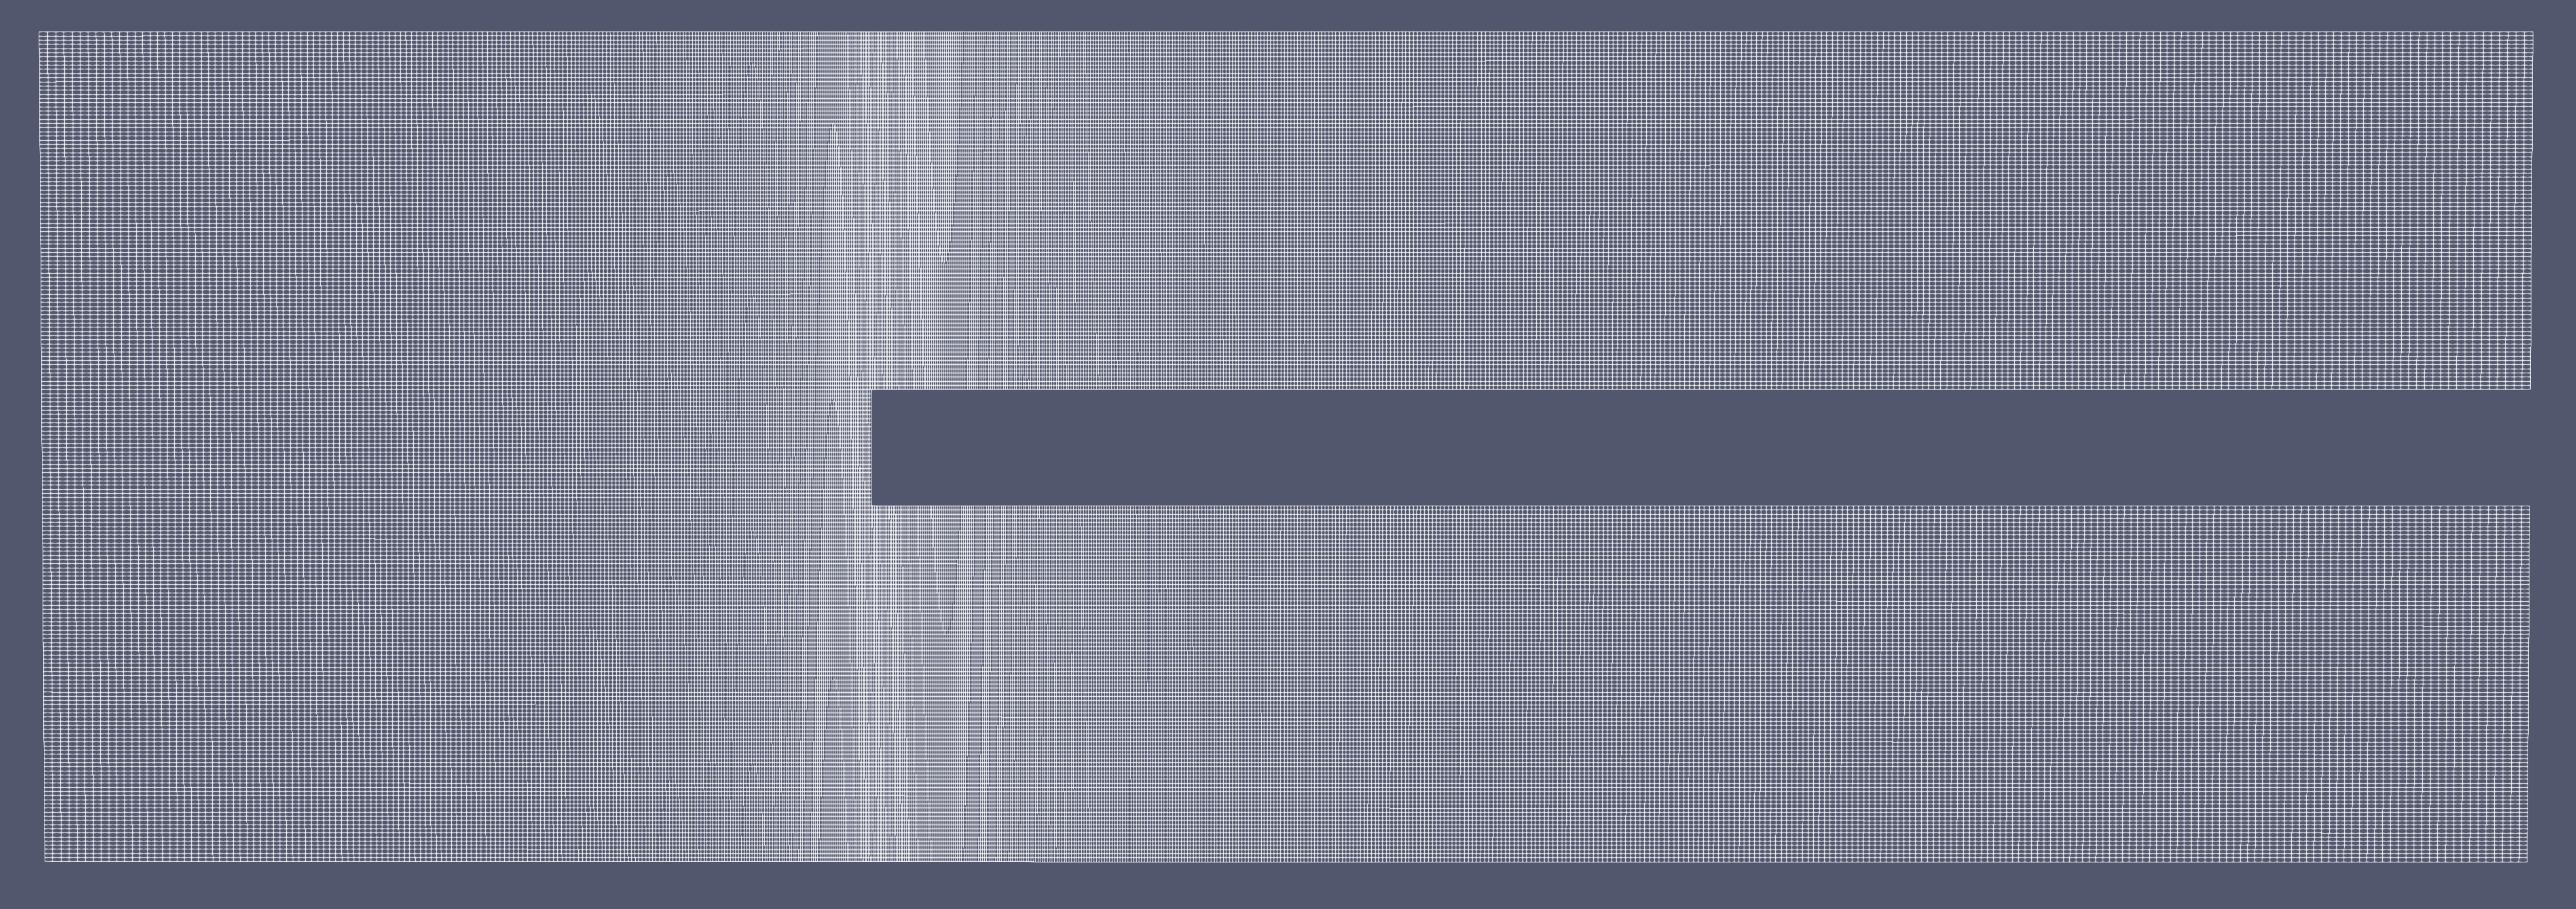
\includegraphics[width=1\linewidth]{pv-mesh.png}
	\caption{Síť řešeného modelu}
	\label{fig:pvmesh}
\end{figure}


Okrajové podmínky pro jednotlivé veličiny, pro nás primárně pro rychlost $U$ a tlak $p$  jsou definovány v souborech ve složce \texttt{0}.

Ostatní parametry řešiče úlohy, netýkající se přímo lineárních řešičů jsou pro všechny simulace totožné a jsou v souborech \texttt{transportProperties}, \texttt{turbulenceProperties}, \texttt{fvSchemes} a \texttt{controlDict}. Zde uvedeme jen vybrané parametry popisující naší úlohu.

\begin{itemize}
	\item{\makebox[5cm]{application:\hfill}simpleFoam}
	\item{\makebox[5cm]{simulationType:\hfill}RAS}
	\item{\makebox[5cm]{RASmodel:\hfill}kEpsilon}
	\item{\makebox[5cm]{turbulence:\hfill}on}
	\item{\makebox[5cm]{transportModel:\hfill}Newtonian}
	\item{\makebox[5cm]{nu:\hfill}1e-05}
	\item{\makebox[5cm]{residualControl p:\hfill}1e-02}
	\item{\makebox[5cm]{residualControl ostatní:\hfill}1e-04}
\end{itemize}


	
Na ukázku je zde obrázek \ref{fig:pv-GAMG-GS} výsledného klidového stavu pořízený v ParaView. Výsledky úlohy řešené pomocí různých lineárních řešičů vypadají prakticky identicky.
	
	 \begin{figure}[H]
		\centering
		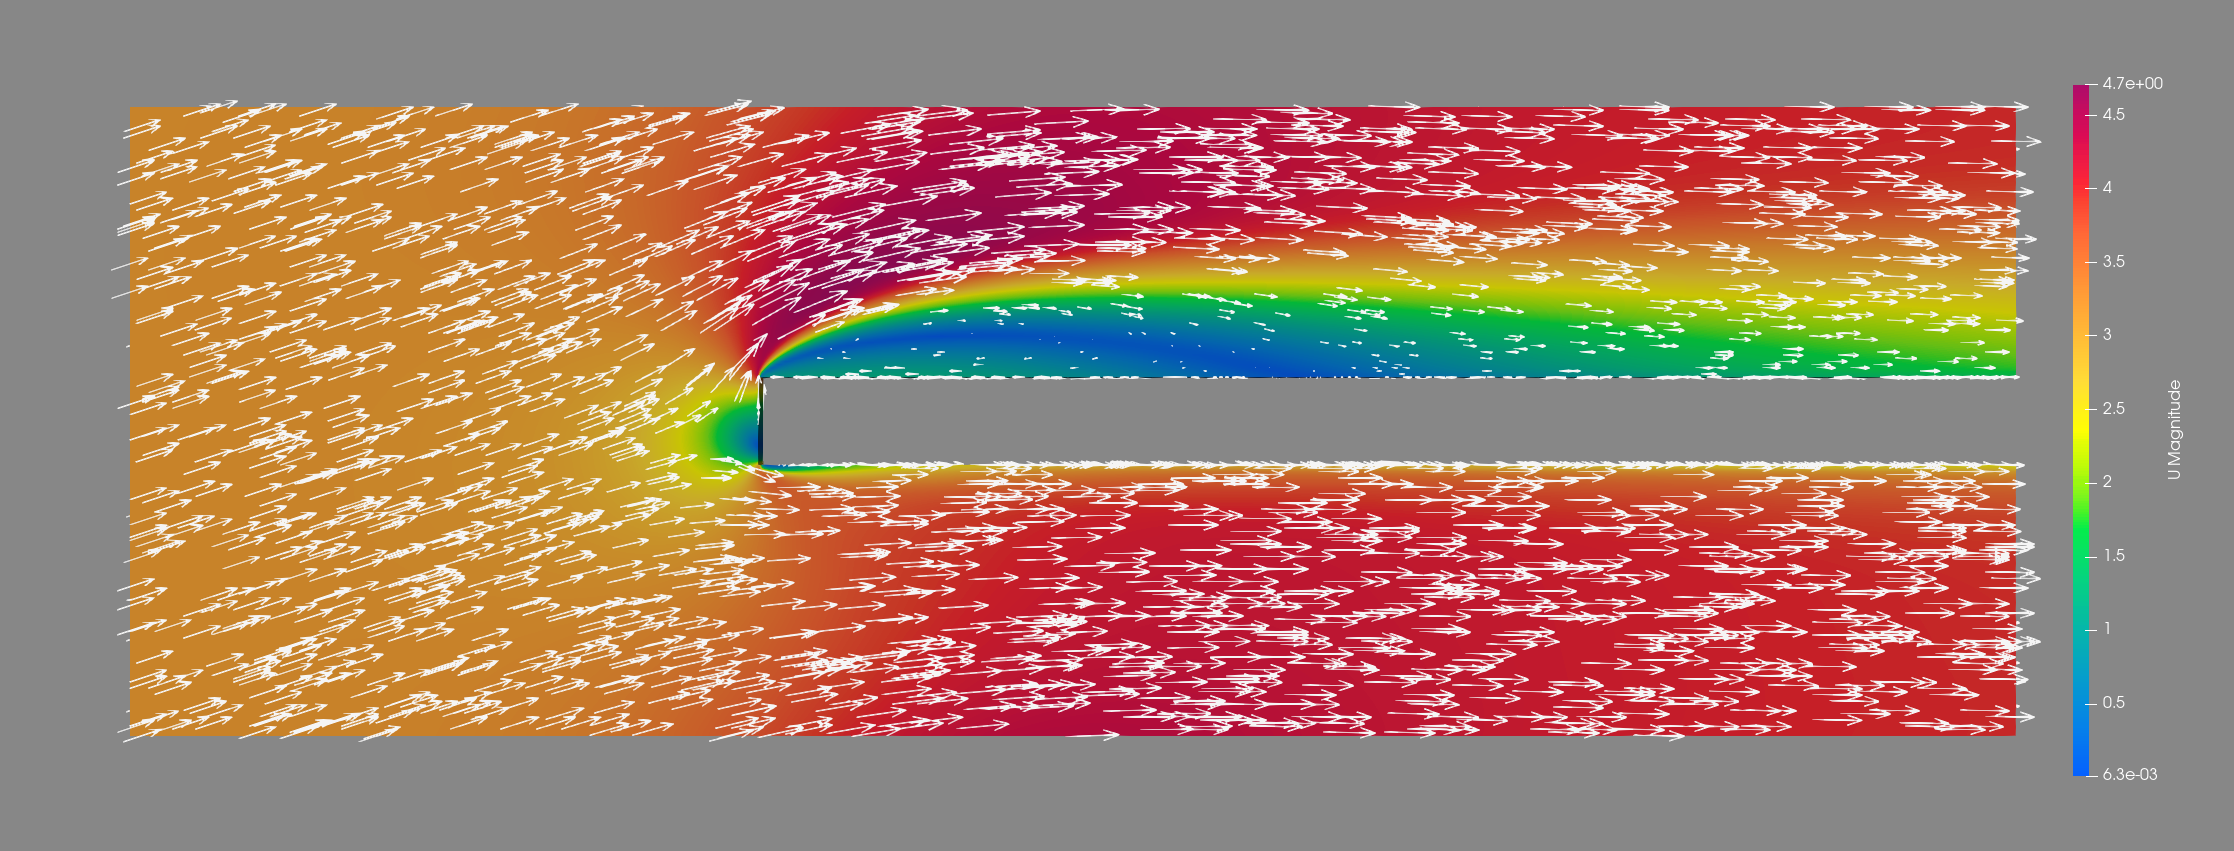
\includegraphics[width=1\linewidth]{pv-GAMG-GS.png}
		\caption{Klidový stav s vektory rychlosti $U$ v ParaView}
		\label{fig:pv-GAMG-GS}
	\end{figure}


Na lineárních řešičích budeme zkoumat vliv následujících parametrů na konvergenci simulace:
 
\begin{itemize}
	\item typ použitého řešiče
	\item typ použitého předpodmiňovače
	\item typ použitého smootheru
	\item hodnotu pod-relaxace
\end{itemize}

Nastavení řešičů se v OpenFOAM dělá v souboru \texttt{system/fvSolution}. Ukázkový soubor je v příloze \ref{app:fvsol}.
	
 Nejprve nás zajímá typ použitého řešiče, případně přidruženého předpodmiňovače nebo smootheru. V tabulkách \ref{table:solvers_GAMG}, \ref{table:solvers_PCG} a \ref{table:solvers_smooth} jsou uvedená nastavení a výsledné počty iterací řešení úlohy a čas běhu simulace testovací úlohy.
 
 Konvergenci metody měříme pomocí počtu využitých iterací metody. Maximální počet iterací byl nastaven na $500$. Tolerance lineárního řešiče je shodně nastavena na $10^{-6}$, relativní tolerance na $0$. Velikost reziduí v rámci SIMPLE algoritmu pomocí \texttt{residualControl} parametru pro tlak $p$ nastaveno na $10^{-3}$ a pro rychlost $U$ na $10^{-4}$.

 \begin{table}[H]
	\centering
	\caption{Nastavení lineárních řešičů pro jednotlivé simulace}
	\renewcommand{\arraystretch}{1.9}
	\begin{tabular}{*7c}
		\toprule
		%\multicolumn{2}{c}{\textbf{Řešič pro $p$}} & \multicolumn{2}{c}{\textbf{Řešič pro $U$}}\\
		\multicolumn{2}{c}{Tlak $p$: \textbf{GAMG}} & \multicolumn{2}{c}{Rychlost $U$: \textbf{GAMG}}\\		
		\midrule
		%\textit{Předpod.}&\textit{Smoother}&\textit{Předpod.}&\textit{Smoother}&\textit{Relaxace}&\textit{ \# iter}&\textit{čas}\\
		Předpod.&Smoother&Předpod.&Smoother&\# iter&Čas\\
		\midrule
 --- & DIC & --- &  DILU & 475 &157.94\\		
 --- & GaussSeidel &  --- & GaussSeidel & 475&176.99\\
		
			\bottomrule
\end{tabular}

\label{table:solvers_GAMG}

\end{table}


\begin{table}[H]
\centering
\caption{Nastavení lineárních řešičů pro jednotlivé simulace}
\renewcommand{\arraystretch}{1.9}
\begin{tabular}{*7c}
\toprule	

%\multicolumn{2}{c}{\textbf{}} & \multicolumn{2}{c}{\textbf{Řešič pro $U$}}\\
\multicolumn{2}{c}{Tlak $p$: \textbf{PCG}} & \multicolumn{2}{c}{Rychlost $U$: \textbf{PBiCG}}\\		
\midrule
%\textit{Předpod.}&\textit{Smoother}&\textit{Předpod.}&\textit{Smoother}&\textit{Relaxace}&\textit{ \# iter}&\textit{čas}\\
Předpod.&Smoother&Předpod.&Smoother&\# iter&Čas\\
\midrule
 DIC & --- &  DILU & --- &474&540.48\\								
FDIC & --- &  DILU & --- &474&531.14\\	
 \shortstack{GAMG\\GS smooth.}& --- &  \shortstack{GAMG\\GS smooth.}& --- &475&184.85\\	
diagonal & --- & diagonal & ---&474&679.26\\	

		\bottomrule
\end{tabular}

\label{table:solvers_PCG}

\end{table}

Z výsledků je patrné, že pro naši úlohu ideální GAMG řešič, což odpovídá i obecným doporučením pro řešení úloh pro klidový stav. PCG/PBiCG řešiče dospějí ke stejným výsledkům, v podobném počtu iterací, jen za víc jak dvojnásobný čas. Obecně al GAMG není tak dobře škálovatelný jaklo PCG/PBiCG a je tedy proto možné, že pro jinou úlohu, případě i stejnou úlohu ale řádově větší síť by mohl být PCG/PBiCG řešič vhodnější.

Na obrázku \ref{fig:p-residuum} jsou zobrazeny průběhy simulací pomocí závislosti velikosti rezidua pro tlak $p$ a různé řešiče. Na obrázku \ref{fig:ux-residuum} je pak totéž, jen pro rychlost v $x$ové souřadnici $U_x$.


\begin{figure}[H]
	\centering
	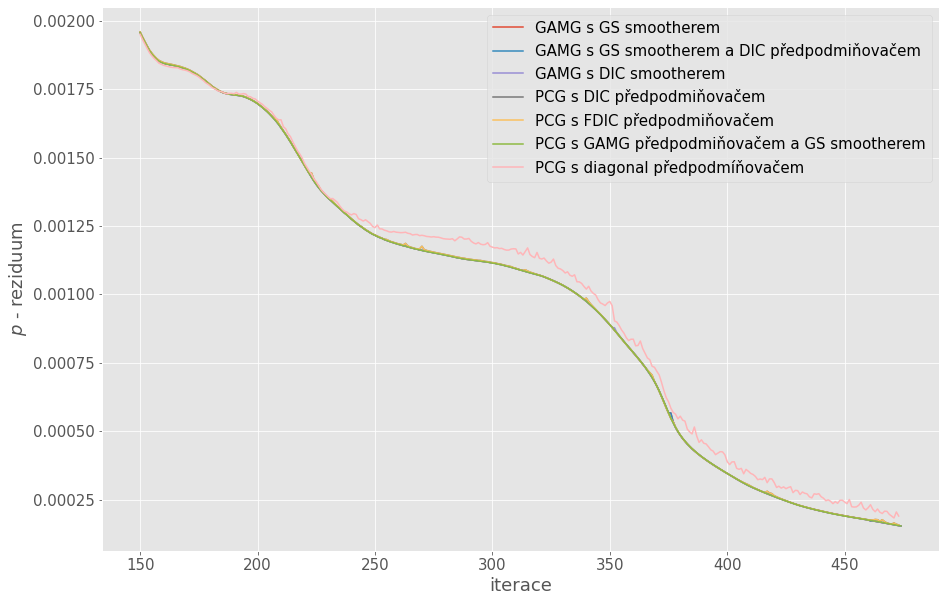
\includegraphics[width=1\linewidth]{p-residuum.png}
	\caption{Konvergence lineárních řešičů v různé konfiguraci pro tlak $p$}
	\label{fig:p-residuum}
\end{figure}


\begin{figure}[H]
	\centering
	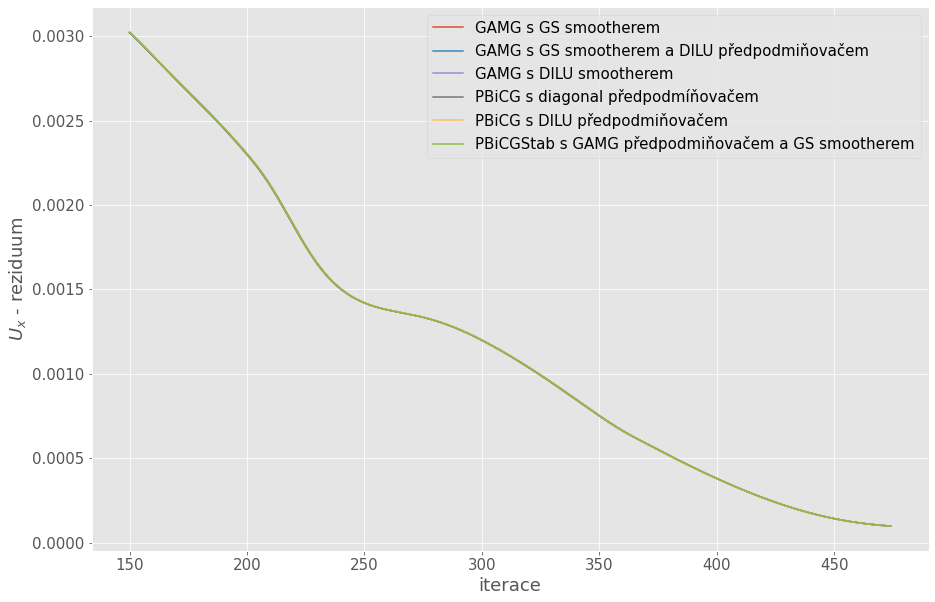
\includegraphics[width=1\linewidth]{ux-residuum.png}
	\caption{Konvergence lineárních řešičů v různé konfiguraci pro rychlost $U_x$}
	\label{fig:ux-residuum}
\end{figure}

Z výsledků v tabulce \ref{table:solvers_smooth} je vidět, že smoothSolver není pro naši úlohu vhodný. Ani v jednom případě nedokonvergovala úloha ke stacionárnímu stavu v stanovém maximálním počtu 500 iterací.  I čas potřebný ke zpracování této úlohy je výrazně vyšší. 

 \begin{table}[H]
	\centering
	\caption{Nastavení lineárních řešičů pro jednotlivé simulace}
	\renewcommand{\arraystretch}{1.9}
	\begin{tabular}{*7c}
		\toprule
\multicolumn{2}{c}{Tlak $p$: \textbf{smoothSolver}} & \multicolumn{2}{c}{Rychlost $U$: \textbf{smoothSolver}}\\
%\multicolumn{2}{c}{\textbf{Řešič pro $p$}} & \multicolumn{2}{c}{\textbf{Řešič pro $U$}}\\
%\multicolumn{2}{c}{\textbf{smoothSolver}} & \multicolumn{2}{c}{\textbf{smoothSolver}}\\		
\midrule
%\textit{Předpod.}&\textit{Smoother}&\textit{Předpod.}&\textit{Smoother}&\textit{Relaxace}&\textit{ \# iter}&\textit{čas}\\
Předpod.&Smoother&Předpod.&Smoother&\# iter&Čas\\
\midrule		
 --- & DIC &  --- & GaussSeidel &500+&1136.21\\	
 --- & DIC & --- & DILU &500+&1039.73\\
 --- & GaussSeidel &   --- & GaussSeidel &500+&1011.42\\		
 FDIC & GaussSeidel &  --- & GaussSeidel &500+&1008.47\\
 --- & \shortstack{symGauss-\\Seidel} &  --- & \shortstack{symGauss-\\Seidel}&500+&1370.58\\	
\bottomrule
\end{tabular}
	
	\label{table:solvers_smooth}
\end{table}

Na obrázcích \ref{fig:p-residuum-smooth} (pro tlak $p$) a \ref{fig:ux-residuum-smooth} (pro rychlost $U_x$) je vidět proč smooth řešič nekonverguje, nebo konverguje velmi pomalu. V obou sledovaných veličinách reziduum osciluje a jeho hodnota se snižuje velmi pomalu.

\begin{figure}[H]
	\centering
	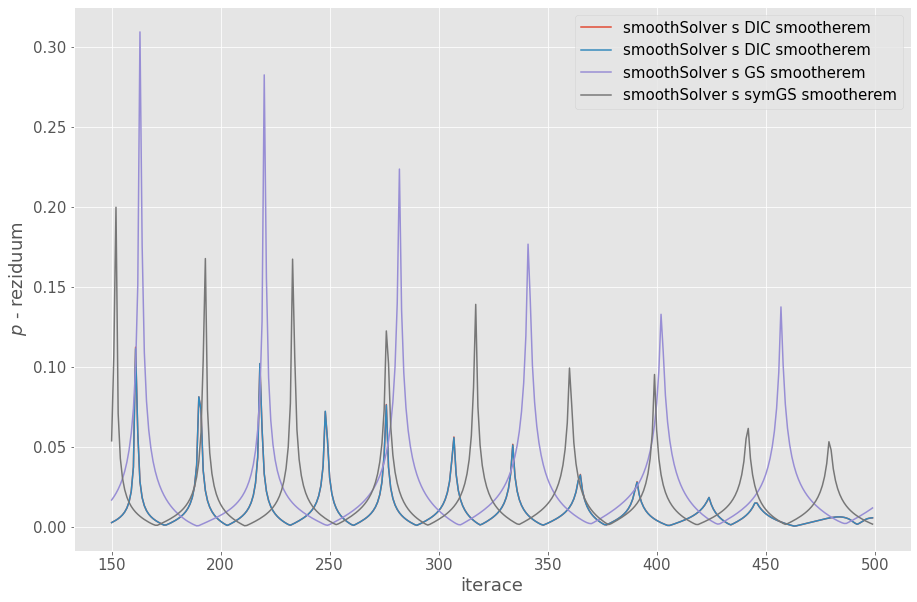
\includegraphics[width=1\linewidth]{p-residuum-smooth.png}
	\caption{Konvergence lineárních řešičů smoothSolver v různé konfiguraci pro tlak $p$}
	\label{fig:p-residuum-smooth}
\end{figure}

\begin{figure}[H]
	\centering
	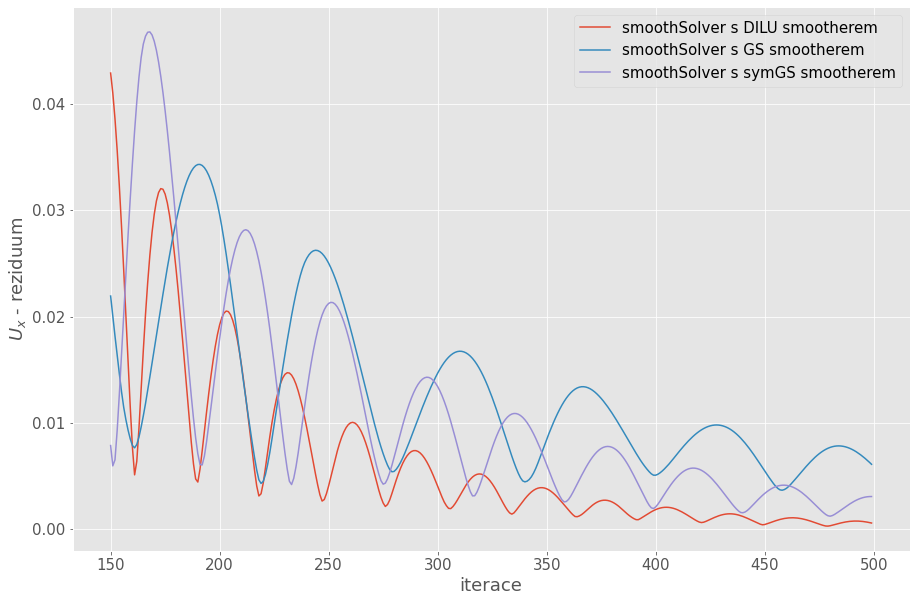
\includegraphics[width=1\linewidth]{ux-residuum-smooth.png}
	\caption{Konvergence lineárních řešičů smoothSolver v různé konfiguraci pro rychlost $U_x$}
	\label{fig:ux-residuum-smooth}
\end{figure}
	


Na GAMG řešiči si ukážeme vliv hodnoty relaxace. Obecně platí, že vyšší relaxace zvyšuje rychlost konvergence, nižší metodu zestabilní. V tabulce \ref{table:solvers_gamg_relax} jsou výsledky pro různé hodnoty relaxačního parametru v porovnání s defaultní hodnotou $0.9$. 

 \begin{table}[H]
	\centering
	\caption{Nastavení lineárních řešičů pro jednotlivé simulace}
	\renewcommand{\arraystretch}{1.9}
	\begin{tabular}{*8c}
		\toprule
		\multicolumn{2}{c}{Tlak $p$: \textbf{GAMG}} & \multicolumn{2}{c}{Rychlost $U$: \textbf{GAMG}}\\		
		\midrule
		%\textit{Předpod.}&\textit{Smoother}&\textit{Předpod.}&\textit{Smoother}&\textit{Relaxace}&\textit{ \# iter}&\textit{čas}\\
		Předpod.&Smoother&Předpod.&Smoother&Relaxace& \# iter&Čas\\
		
		\midrule
		
		--- & GaussSeidel &  --- & GaussSeidel & 0.9&475&176.99\\
		--- & GaussSeidel &  --- & GaussSeidel & 0.3&500+&151.49\\
		--- & GaussSeidel &  --- & GaussSeidel & 0.95&285&114.15\\
		--- & GaussSeidel &  --- & GaussSeidel & 0.98&500+&257.28\\		
		%%%%DIC & GaussSeidel &  DILU & GaussSeidel & 0.98&475&160.59\\
		\bottomrule
	\end{tabular}
	
	\label{table:solvers_gamg_relax}
	
\end{table}

Ideální hodnotou pro nejrychlejší konvergenci je $0.95$, úloha dokoverguje v 285 iteracích za přibližně $114s$. Hodnota relaxace $0.3$ je moc nízká na to, aby úloha dokonvergovala v maximálním počtu 500 iterací.  Hodnota $0.98$ je naopak moc vysoká a reziduum úlohy se rozkmitá a řešení nekonverguje, jak je vidět z obrázků \ref{fig:p-residuum-relax} a \ref{fig:ux-residuum-relax}.

\begin{figure}[H]
	\centering
	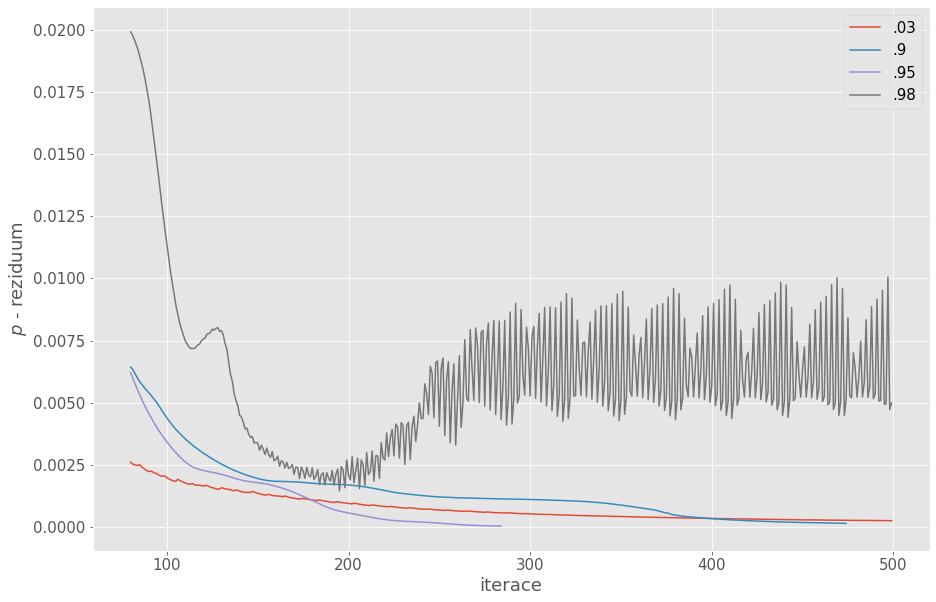
\includegraphics[width=1\linewidth]{p-under-relax.png}
	\caption{Konvergence lineárních řešičů smoothSolver v různé konfiguraci pro rychlost $U_x$}
	\label{fig:p-residuum-relax}
\end{figure}

\begin{figure}[H]
	\centering
	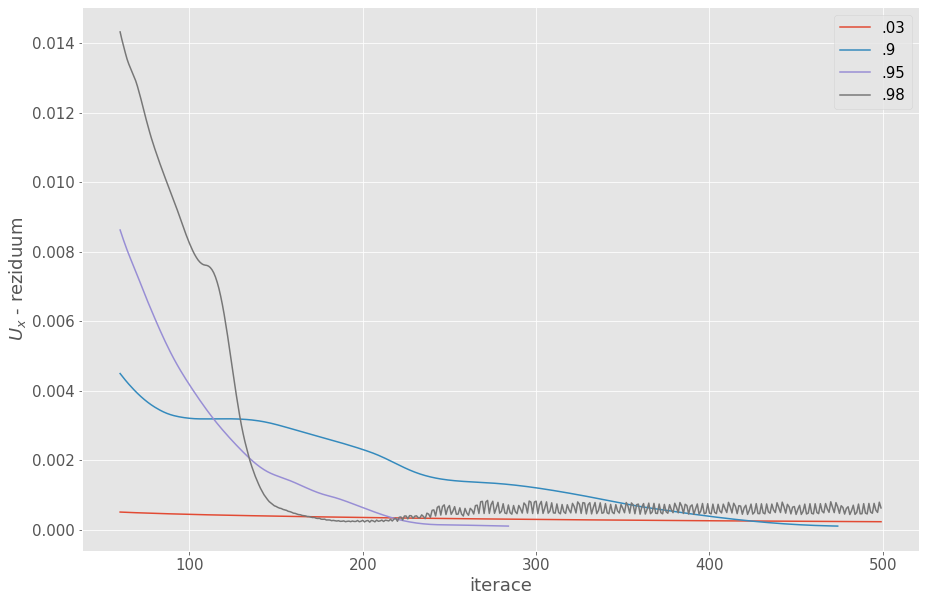
\includegraphics[width=1\linewidth]{ux-under-relax.png}
	\caption{Konvergence lineárních řešičů smoothSolver v různé konfiguraci pro rychlost $U_x$}
	\label{fig:ux-residuum-relax}
\end{figure}

Zdálo by se, že použít relaxaci na \uv{opravení} smooth řešiče je dobrý nápad. Z tabulky \ref{table:solvers_set3}  je ale vidět, že se výsledky nijak nezlepší.

\begin{table}[H]
	\centering
	\caption{Nastavení lineárních řešičů pro jednotlivé simulace}
	\renewcommand{\arraystretch}{1.9}
	\begin{tabular}{*8c}
		\toprule
		\multicolumn{2}{c}{Tlak $p$: \textbf{smoothSolver}} & \multicolumn{2}{c}{Rychlost $U$: \textbf{smoothSolver}}\\
		\midrule
		%\textit{Předpod.}&\textit{Smoother}&\textit{Předpod.}&\textit{Smoother}&\textit{Relaxace}&\textit{ \# iter}&\textit{čas}\\
		Předpod.&Smoother&Předpod.&Smoother&Relaxace& \# iter&Čas\\
		\midrule
		--- & GaussSeidel &   --- & GaussSeidel &0.9&500+&1011.42\\
		--- & GaussSeidel &  --- & GaussSeidel &0.3&500+&951.71\\
		--- & GaussSeidel &   --- & GaussSeidel &0.95&500+&1086.7\\
		--- & GaussSeidel &  --- & GaussSeidel &0.98&500+&1222.24\\
		FDIC & GaussSeidel &  --- & GaussSeidel &0.9&500+&1008.47\\
		\bottomrule
	\end{tabular}
	
	\label{table:solvers_set3}
\end{table}

Další parametr, který popíše \uv{úspěšnost} lineárního řešiče při řešení úlohy je počet iteračních kroků lineárního řešiče v rámci časových kroků metody. V každém kroku řeší lineární řešič soustavu a zastaví iterování v chvíli, kdy dosáhne nastavené tolerance. Na obrázcích \ref{fig:p-iters-1} a \ref{fig:p-iters-2} je vidět tato závislost pro řešení tlaku $p$, na obrázku \ref{fig:ux-iters} pak pro rychlost $U_x$. Ze všech tří grafů opět vyplývá, že GAMG řešič dosahuje nejlepší konvergence. Naopak smoothSolver naráží ve všech časových iterací metody na maximální možnou hodnotu iterací řešiče $1000$.

\begin{figure}[H]
	\centering
	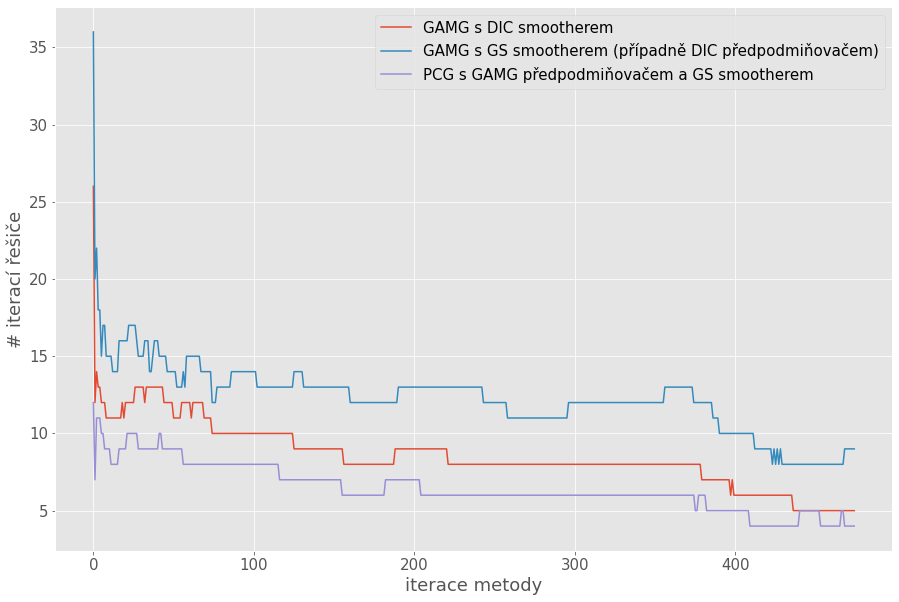
\includegraphics[width=1\linewidth]{p-solver-iters-1.png}
	\caption{Počet iterací lineárního řešiče v závislosti na iteraci metody pro tlak $p$}
	\label{fig:p-iters-1}
\end{figure}

\begin{figure}[H]
	\centering
	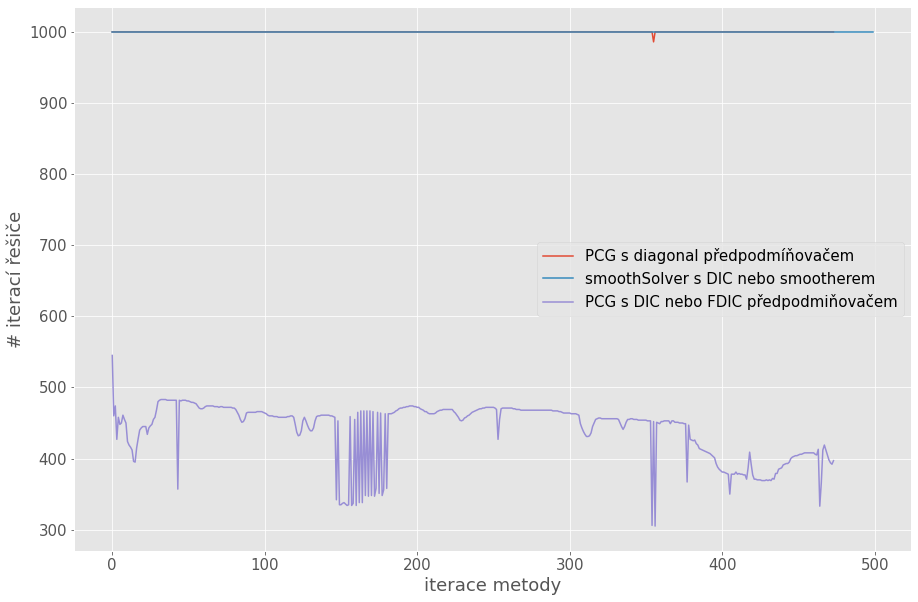
\includegraphics[width=1\linewidth]{p-solver-iters-2.png}
	\caption{Počet iterací lineárního řešiče v závislosti na iteraci metody pro tlak $p$}
	\label{fig:p-iters-2}
\end{figure}

\begin{figure}[H]
	\centering
	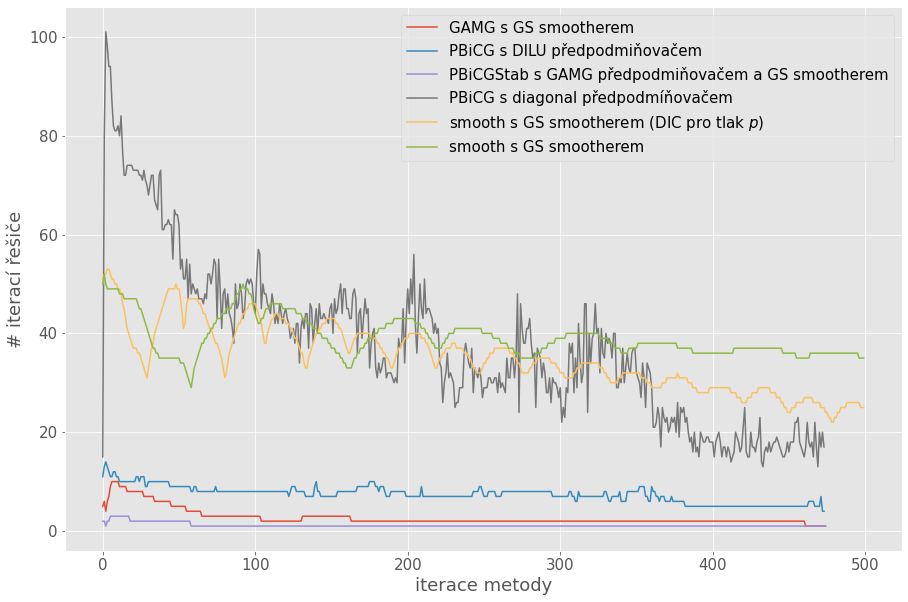
\includegraphics[width=1\linewidth]{ux-solver-iters.png}
	\caption{Počet iterací lineárního řešiče v závislosti na iteraci metody pro rychlost $U_x$}
	\label{fig:ux-iters}
\end{figure}



{\let\clearpage\relax \chapter{Závěr}}

Ukázali jsme, jakými parametry lineárních řešičů se dá ovlivnit výsledná konvergence úlohy. Obecně nelze říci, který řešič je nejvhodnější a to ani pro konkrétní úlohu. Pro naši ukázkovou úlohu proudění v lopatkové mříži a pro konkrétní síť je nejvhodnější GAMG řešič s GaussSeidel smootherem a relaxací nastavenou na $0.95$. Tato volba ale nemusí být optimální pro jinou síť, jinak nastavené parametry turbulence nebo i jiný hardware, na kterém úlohu řešíme. Předchozí text by tedy měl sloužit přinejlepším jen jako přehled a ukázka řešičů dostupných v OpenFOAM.



\newpage
\appendix

{\let\clearpage\relax \chapter{blockMeshDict}\label{app:blockmeshdict}}
\begin{verbatim}
/*---------------------------*- C++ -*-----------------------------*\
| =========                 |                                                 |
| \\      /  F ield         | OpenFOAM: The Open Source CFD Toolbox           |
|  \\    /   O peration     | Version:  v2006                                 |
|   \\  /    A nd           | Website:  www.openfoam.com                      |
|    \\/     M anipulation  |                                                 |
\*-----------------------------------------------------------------*/
FoamFile
{
	version         2.0;
	format          ascii;
	class           dictionary;
	object          blockMeshDict;
}
// * * * * * * * * * * * * * * * * * * * * * * * * * * * * * * * * //

scale   1;

vertices
(
(0 0    0)
(1 0    0)
(3 0    0)
(3 0.43 0)
(1 0.43 0)
(1 0.57 0)
(3 0.57 0)
(3 1    0)
(1 1    0)
(0 1    0)
(0 0.57 0)
(0 0.43 0)


(0 0    0.1)
(1 0    0.1)
(3 0    0.1)
(3 0.43 0.1)
(1 0.43 0.1)
(1 0.57 0.1)
(3 0.57 0.1)
(3 1    0.1)
(1 1    0.1)
(0 1    0.1)
(0 0.57 0.1)
(0 0.43 0.1)


);

blocks
(
hex (0 1 4 11 12 13 16 23) (200 86 1) simpleGrading (0.2 1 1)
hex (1 2 3 4 13 14 15 16) (400 86 1) simpleGrading (5 1 1)
hex (11 4 5 10 23 16 17 22) (200 28 1) simpleGrading (0.2 1 1)
hex (10 5 8 9 22 17 20 21) (200 86 1) simpleGrading (0.2 1 1)
hex (5 6 7 8 17 18 19 20) (400 86 1) simpleGrading (5 1 1)
);

edges
(
);

boundary
(
frontAndBack
{
	type empty;
	faces
	(
	(0 1 4 11)
	(1 2 3 4)
	(11 4 5 10)
	(10 5 8 9)
	(5 6 7 8)
	
	(12 13 16 23)
	(13 14 15 16)
	(23 16 17 22)
	(22 17 20 21)
	(17 18 19 20)
	);
}

top	
{
	type cyclic;
	neighbourPatch bottom;
	faces
	(
	(9 8 20 21)
	(8 7 19 20)
	);
}

bottom	
{
	type cyclic;
	neighbourPatch top;
	faces
	(
	(0 1 13 12)
	(1 2 14 13)
	);
}

fixedBalk
{
	type wall;
	faces
	(
	(5 6 18 17)
	(4 5 17 16)
	(4 3 15 16)
	);	
}

outlet
{
	type patch;
	faces
	(
	(6 7 19 18)
	(2 3 15 14)
	);
}

inlet
{
	type patch;
	faces
	(
	(0 11 23 12)
	(11 10 22 23)
	(10 9 21 22)
	);
}
);
mergePatchPairs
(
);

// ************************************************************** //
\end{verbatim}

{\let\clearpage\relax \chapter{fvSolution}\label{app:fvsol}}
\begin{verbatim}
	/*---------------------------*- C++ -*-----------------------------*\
	| =========                 |                                                 |
	| \\      /  F ield         | OpenFOAM: The Open Source CFD Toolbox           |
	|  \\    /   O peration     | Version:  v2006                                 |
	|   \\  /    A nd           | Website:  www.openfoam.com                      |
	|    \\/     M anipulation  |                                                 |
	\*-----------------------------------------------------------------*/
	FoamFile
	{
		version     2.0;
		format      ascii;
		class       dictionary;
		location    "system";
		object      fvSolution;
	}
	// * * * * * * * * * * * * * * * * * * * * * * * * * * * * * * * * //
	
	solvers
	{
		p
		{
			solver          smoothSolver;
			smoother        GaussSeidel;
			tolerance       1e-06;
			relTol          0; 
		}
		
		"(U|k|epsilon|omega|f|v2)"
		{
			solver          smoothSolver;
			smoother        GaussSeidel;
			tolerance       1e-06;
			relTol          0; 
		}
	}
	
	SIMPLE
	{
		nNonOrthogonalCorrectors 0;
		consistent      yes;
		
		residualControl
		{
			p               1e-3;
			U               1e-4;
			"(k|epsilon|omega|f|v2)" 1e-4;
		}
	}
	
	relaxationFactors
	{
		equations
		{
			U               .95; 
			".*"            .95;
		}
	}
	
	
	// ************************************************************** //
\end{verbatim}
	
\end{document}